\documentclass[a4paper,12pt]{article}
\usepackage[T2A]{fontenc}
\usepackage[utf8]{inputenc}
\usepackage[english,russian]{babel}
\usepackage{listings}

\usepackage{amsmath}
\usepackage{MnSymbol}
\usepackage{wasysym}
\usepackage{indentfirst}
\usepackage[unicode, pdftex]{hyperref}

\usepackage{pgfplots}
\pgfplotsset{compat=1.9}

\usepackage{geometry}
\geometry{left=2cm}
\geometry{right=1.5cm}
\geometry{top=1cm}
\geometry{bottom=2cm}

\usepackage{graphicx}
\graphicspath{{img/}}
\DeclareGraphicsExtensions{.pdf,.png,.jpg}

\usepackage{float}

\newcommand{\anonsection}[1]{\section*{#1}\addcontentsline{toc}{section}{#1}}

% переименовываем  список литературы в "список используемой литературы"
\addto\captionsrussian{\def\refname{Список используемой литературы}}

\lstset{
    language=C++,
    numbers=left,
    frame=single,
    texcl=true,
    basicstyle=\ttfamily
}

\begin{document}

\begin{titlepage}

    \begin{center}
        \large
        Государственное образовательное учреждение высшего профессионального образования\\
        “Московский государственный технический университет имени Н.Э.Баумана”
        \vspace{3cm}

        \textsc{Дисциплина: Анализ алгоритмов}
        \vspace{0.5cm}

        \textsc{Лабораторная работа №2}
        \vspace{3cm}

        {\LARGE ТРУДОЕМКОСТЬ АЛГОРИТМОВ УМНОЖЕНИЯ МАТРИЦ}
        \vspace{3cm}

        Студент группы ИУ7-53,\\
        Степанов Александр Олегович
        \vfill
    \end{center}

    \begin{flushright}
        \begin{tabular}{l}
            Преподаватели:\\
            Строганов Юрий Владимирович\\
            Волкова Лилия Леонидовна
        \end{tabular}
    \end{flushright}

    \begin{center}

        2019 г.

    \end{center}

\end{titlepage}

\tableofcontents

\newpage
\anonsection{Введение}

Умножение матриц является основным инструментом линейной алгебры и имеет
многочисленные применения в математике, физике, программировании \cite{haskell}.

В данной лабораторной работе ставятся следующие задачи:

\begin{enumerate}
    \item изучение алгоритмов умножения матриц;
    \item сравнительный анализ стандартного алгоритма и улучшенных алгоритмов по
        затрачиваемым ресурсам;
    \item экспериментальное подтверждение различий во временной эффективности
        сравниваемых алгоритмов.
\end{enumerate}

\newpage
\section{Аналитическая часть}

Умножение матриц активно применяется в областях физики, математики и программирования.
Рассмотрим как можно решить эту задачу.

\subsection{Описание задачи}

Пусть даны две прямоугольные матрицы $A$ и $B$ размерности $l \times m$ и $m \times n$
соответственно, указанные в формуле \ref{ab}.

\begin{equation}\label{ab}
    A =
    \left[
        \begin{matrix}
            a_{11} & a_{12} & \cdots & a_{1m} \\
            a_{21} & a_{22} & \cdots & a_{2m} \\
            \vdots & \vdots & \ddots & \vdots \\
            a_{l1} & a_{l2} & \cdots & a_{lm} \\
        \end{matrix}
    \right],
    B =
    \left[
        \begin{matrix}
            b_{11} & b_{12} & \cdots & b_{1n} \\
            b_{21} & b_{22} & \cdots & b_{2n} \\
            \vdots & \vdots & \ddots & \vdots \\
            b_{m1} & b_{m2} & \cdots & b_{mn} \\
        \end{matrix}
    \right]
\end{equation}

Тогда матрица $C$ будет размерностью $l \times n$ в формуле \ref{c}, в которой
каждый элемент равен выражению из формулы \ref{res} \cite{litr}.

\begin{equation}\label{c}
    C =
    \left[
        \begin{matrix}
            c_{11} & c_{12} & \cdots & c_{1n} \\
            c_{21} & c_{22} & \cdots & c_{2n} \\
            \vdots & \vdots & \ddots & \vdots \\
            c_{l1} & c_{l2} & \cdots & c_{ln} \\
        \end{matrix}
    \right]
\end{equation}

\begin{equation}\label{res}
    c_{ij} = \sum_{k=1}^m a_{ik} \cdot b_{kj}, i = \overline{1;l}, j = \overline{1;n}
\end{equation}

Операция умножения двух матриц выполнима только в том случае, если число столбцов в
первом сомножителе равно числу строк во втором; в этом случае говорят, что матрицы
согласованы. В частности, умножение всегда выполнимо, если оба сомножителя —
квадратные матрицы одного и того же порядка \cite{litr}.

Таким образом, из существования произведения $A \times B$ вовсе не следует
существование произведения $B \times A$ \cite{litr}.

Помимо обычного перемножения матриц по формуле существуют модификации, работающие
быстрее. Рассмотрим в данной лабораторной работе алгоритм Винограда, являющийся одним
из самых эффективных по времени алгоритмов умножения матриц \cite{haskell},
и ее оптимизацию. Этот алгоритм основывается на подготовке вычислений перед вычислением
результирующей матрицы. Если разложить формулу \ref{res} на суммы, то получается
результат, видимый на формуле \ref{vinres}.

\begin{equation}\label{vinres}
    c_{ij} =
    \sum_{k=1}^{\frac{n}{2}} (a_{i,2k-1} + b_{2k,j}) \cdot (a_{i,2k} + b_{2k-1,j}) -
    \underbrace{\sum_{k=1}^{\frac{n}{2}} a_{i,2k-1} \cdot a_{i,2k} -
    \sum_{k=1}^{\frac{n}{2}} b_{2k-1,j} \cdot b_{2k,j}}_\text{Можно вычислить заранее}
\end{equation}

Таким образом, можно заранее вычислить две последние суммы, поскольку они вычисляются
многократно для каждой строки в одном столбце в случае первой и для каждого столбца
из одной строки в случае второй сумм, что уменьшает долю умножения\cite{haskell}.

\subsection{Выводы}

Умножение матриц необходимый инструмент, для которого есть пути ускорения вычислений
за счет уменьшения доли умножения.

\newpage
\section{Конструкторская часть}

Рассмотрим стандартный алгоритм умножения матриц, алгоритм Винограда и улучшенный
алгоритм Винограда.

\subsection{Функциональная модель}

На рисунке \ref{img:idef0} представлена функциональная модель IDEF0 уровня 1.

\begin{figure}[H]
    \center{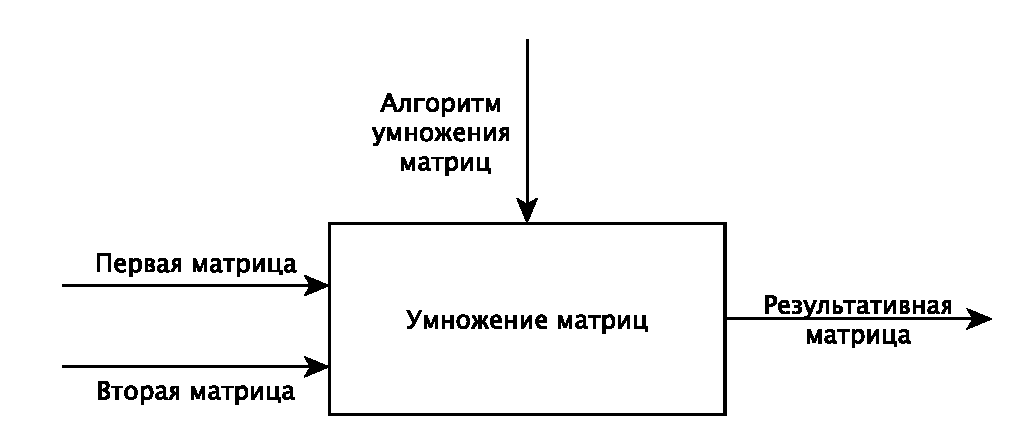
\includegraphics[scale=0.8]{IDEF0}}
    \caption{Функциональная модель IDEF0 уровня 1}
    \label{img:idef0}
\end{figure}

\subsection{Схемы алгоритмов}

На рисунке \ref{img:default} изображена схема стандартного алгоритма произведения
матриц

\begin{figure}[H]
    \center{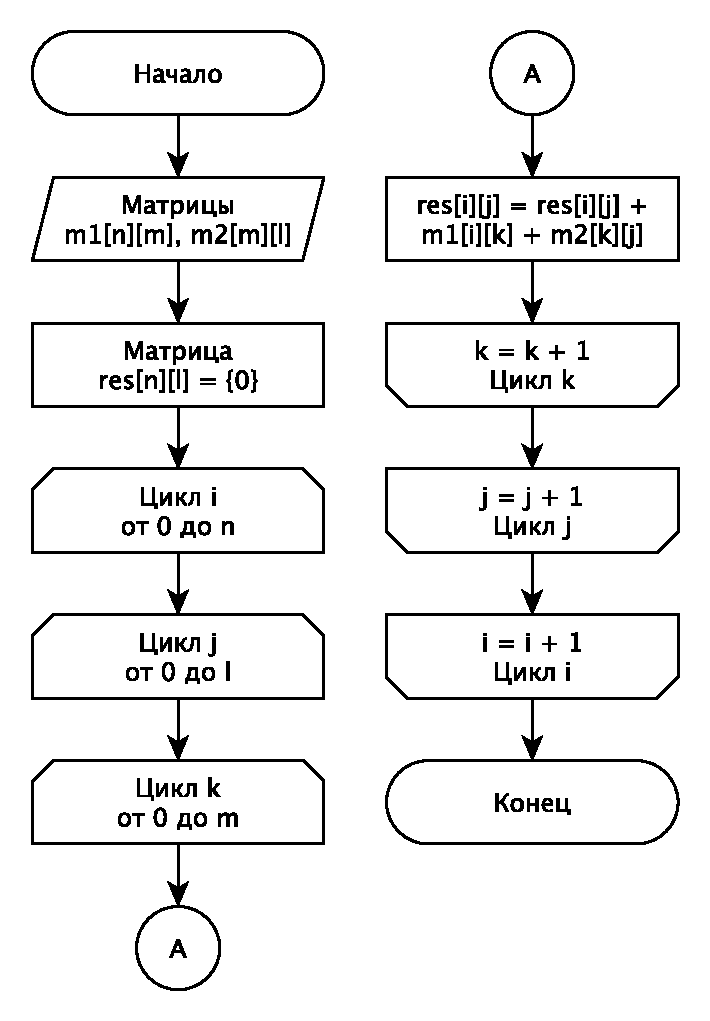
\includegraphics[scale=0.65]{default}}
    \caption{Схема стандартного алгоритма}
    \label{img:default}
\end{figure}

На рисунке \ref{img:vinograd} изображена схема алгоритма
Винограда произведения матриц

\begin{figure}[H]
    \center{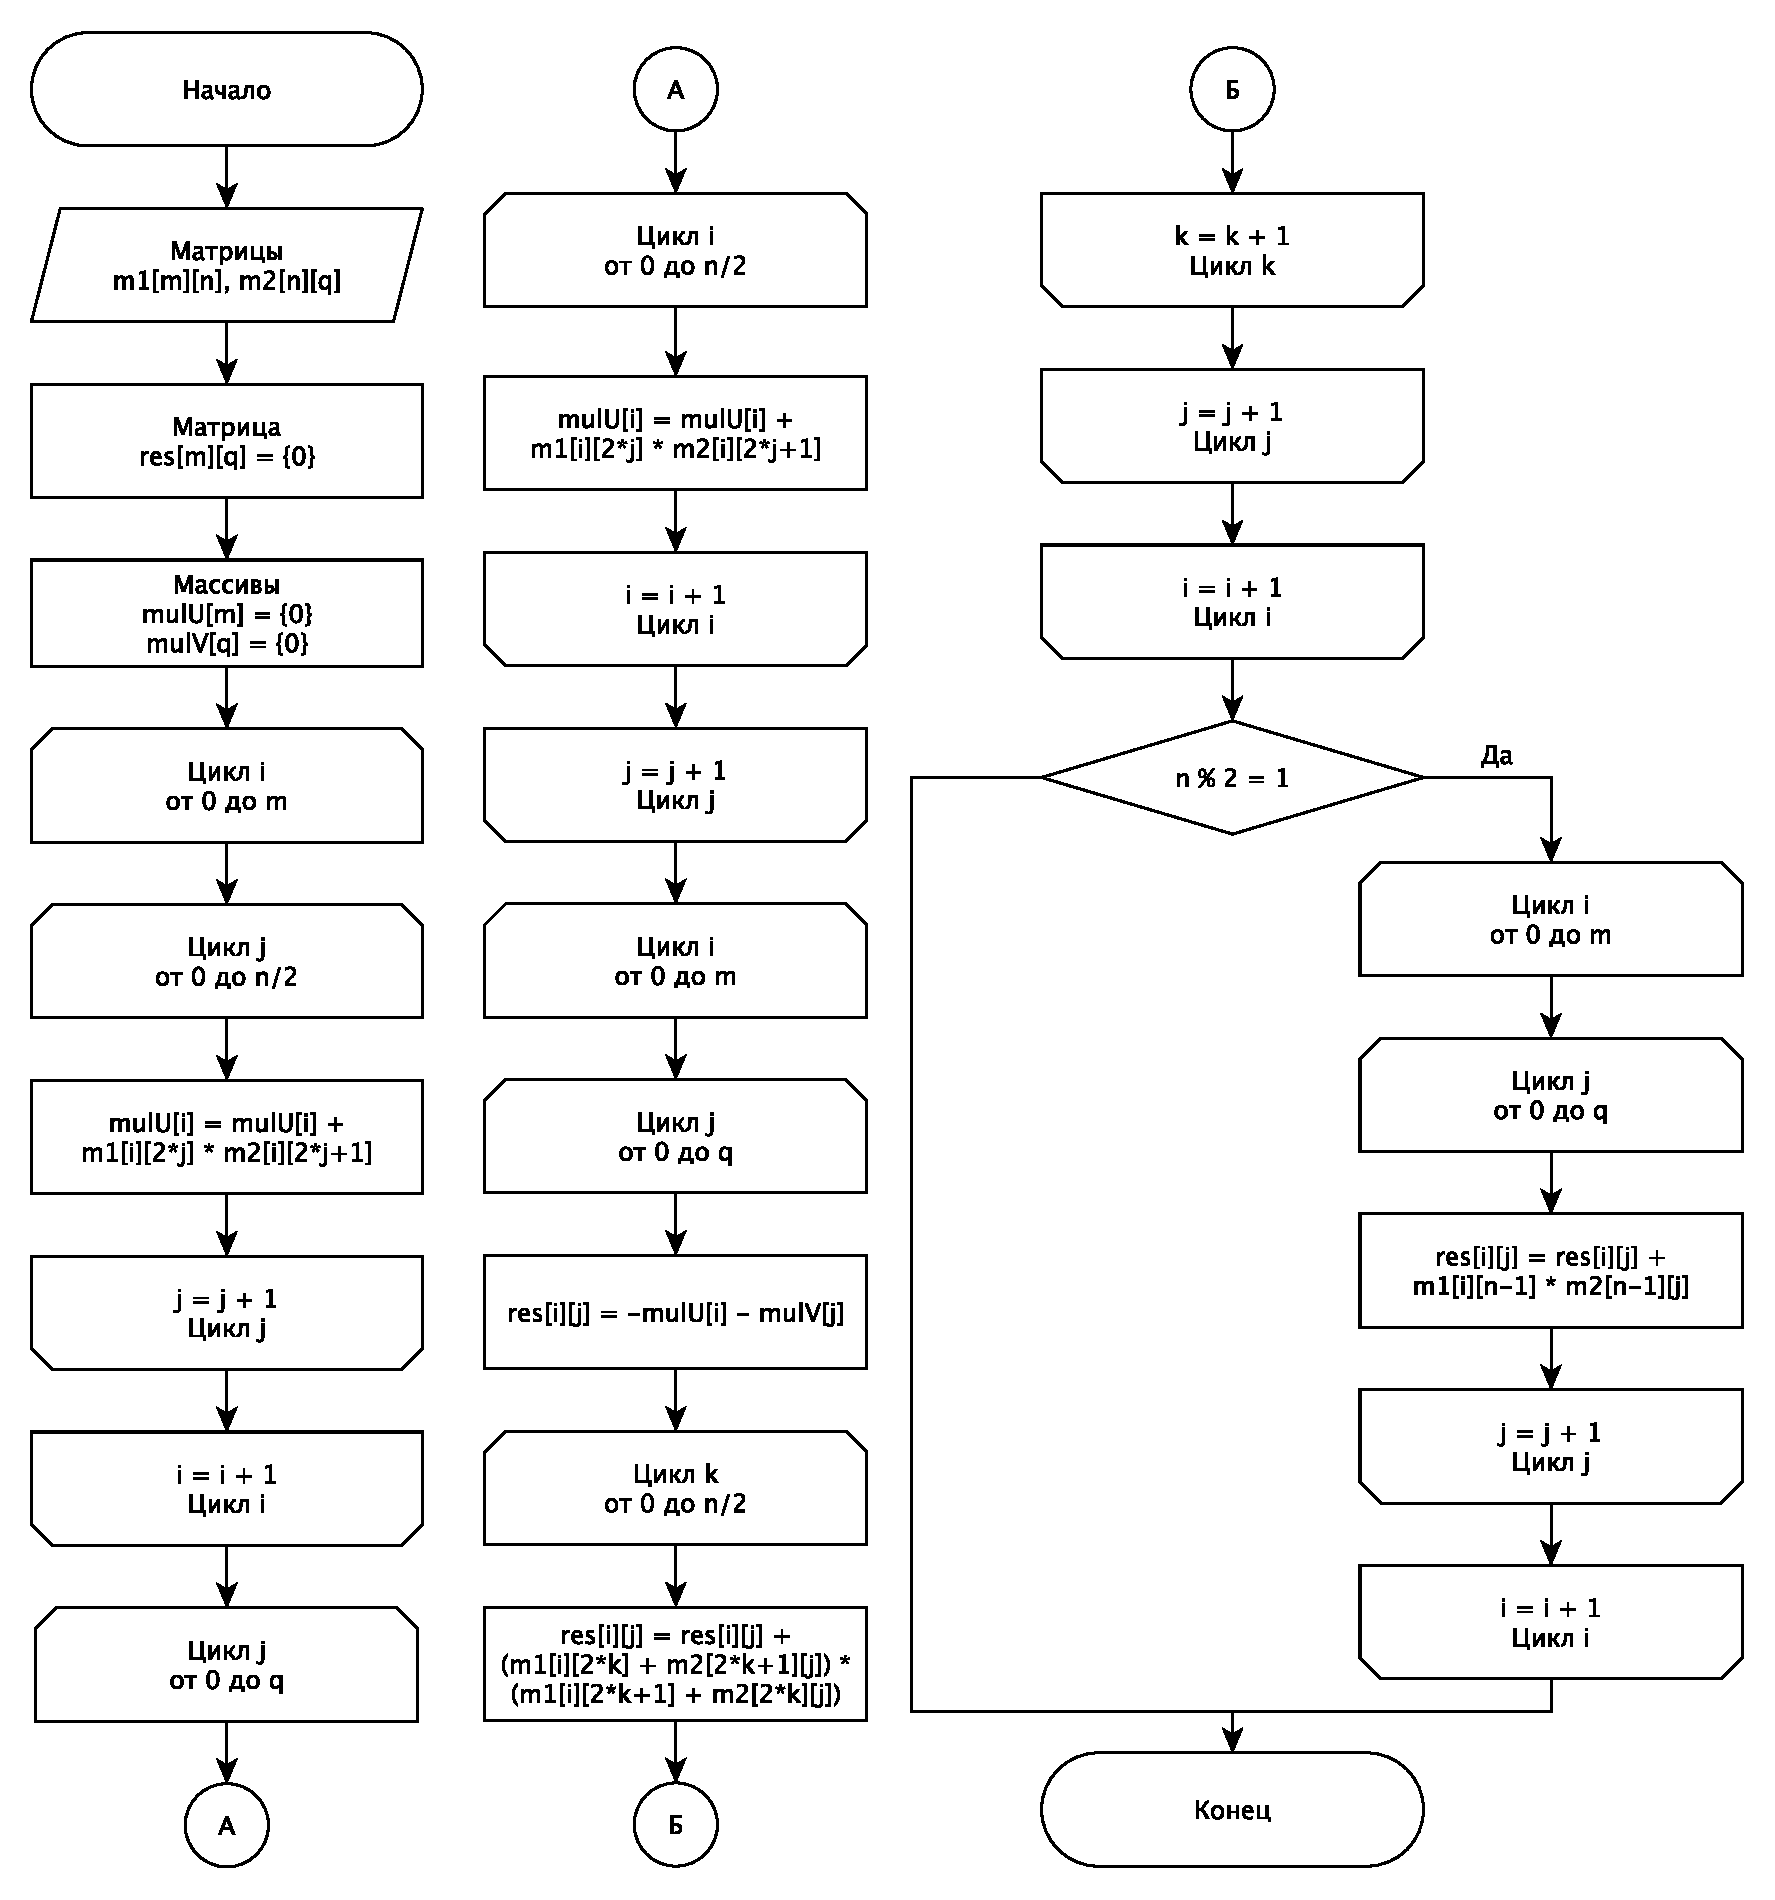
\includegraphics[scale=0.6]{vinograd}}
    \caption{Схема алгоритма Винограда}
    \label{img:vinograd}
\end{figure}

На рисунке \ref{img:modvinograd} изображена схема
оптимизированного алгоритма Винограда. Его удалось оптимизировать в трех местах:

\begin{itemize}
    \item {\ttfamily mulU} и {\ttfamily mulV} сразу ищутся с отрицательным знаком;
    \item для прибавления выражений к переменной используется оператор {\ttfamily +=};
    \item вместо цикла до $\frac{n}{2}$ происходит прибавление к переменной цикла
        по 2, а не по 1.
\end{itemize}

\begin{figure}[H]
    \center{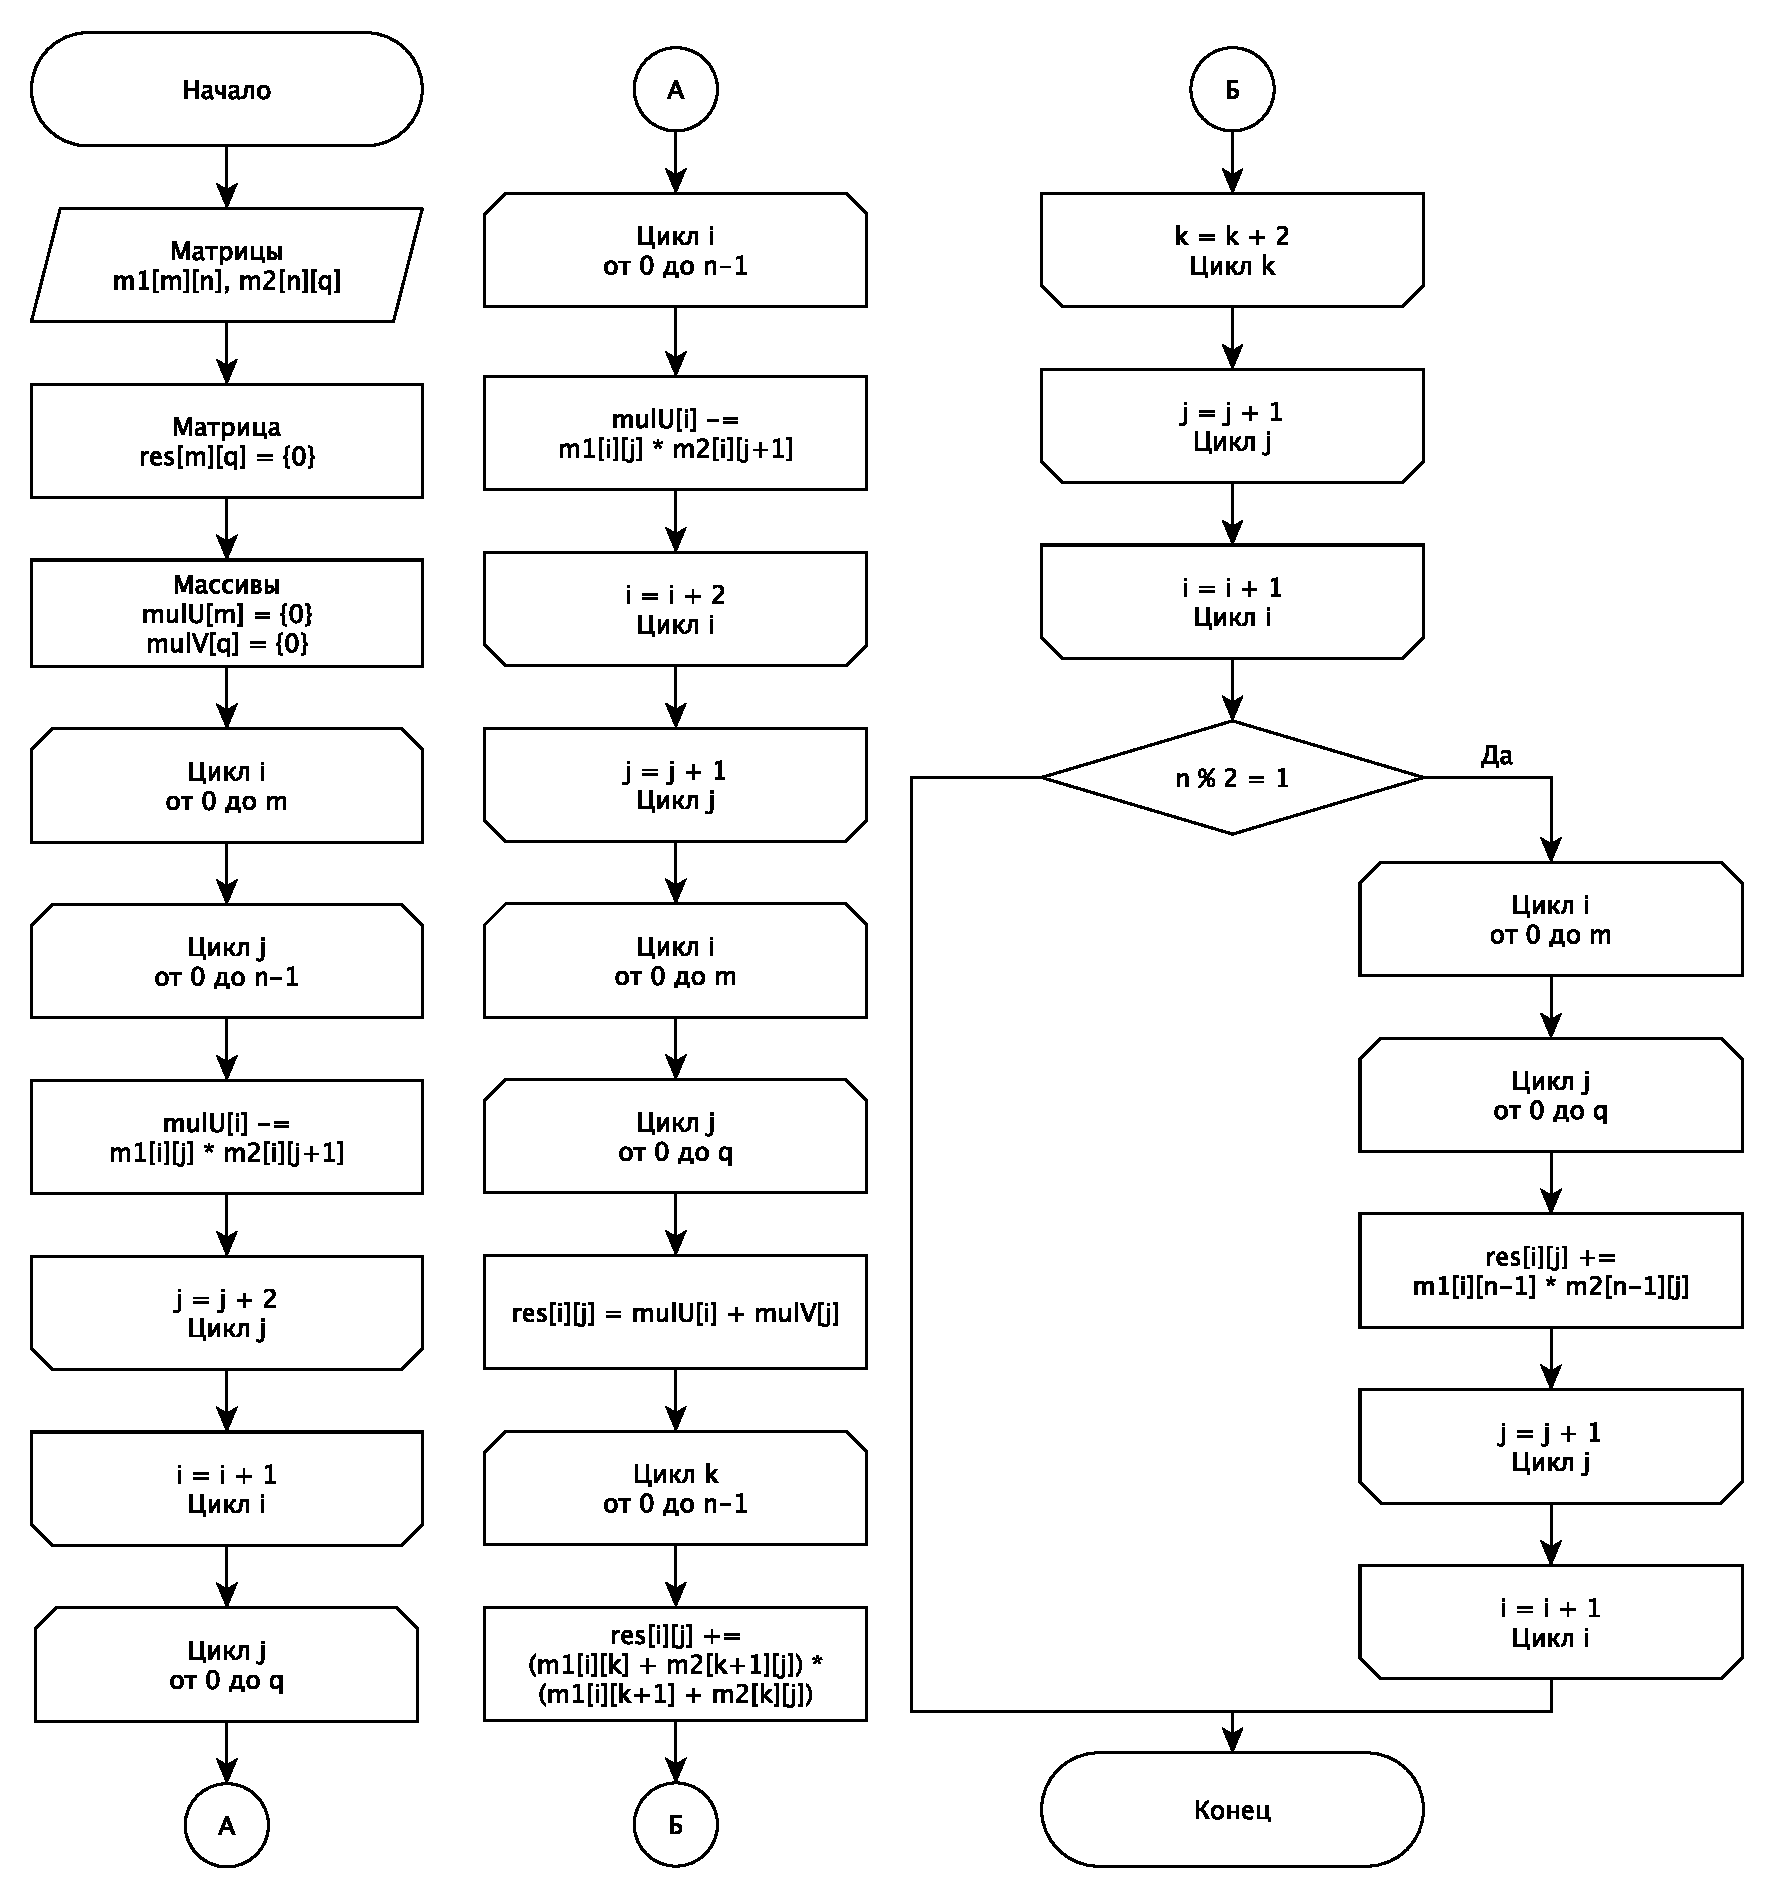
\includegraphics[scale=0.6]{modvinograd}}
    \caption{Схема оптимизированного алгоритма Винограда}
    \label{img:modvinograd}
\end{figure}

Произведем теоретическую оценку трудоемкости алгоритмов умножения матриц

\begin{enumerate}
    \item Стандартный алгоритм

        \begin{equation}
            f = 2 + M(2 + 2 + Q(2 + 2 + N(2 + 8 + 1 + 1 + 1))) =
            13MNQ + 4MQ + 4M + 2
        \end{equation}

    \item Алгоритм Винограда

        \begin{equation}
            f = 2 + M(2 + 2 + Q(2 + 4 + 3 + 3 + \frac{N}{2}(3 + 12 + 11))) =
            13MNQ + 12MQ + 4M + 2
        \end{equation}

        Но доля умножения меньше, чем в стандартном.

    \item Алгоритм Винограда с оптимизацией

        После введенных оптимизаций трудоемкость будет в формуле \ref{modvineff}.

        \begin{equation}\label{modvineff}
            f = 2 + M(2 + 2 + Q(2 + 6 + 2 + \frac{N}{2}(2 + 3 + 7 + 6))) =
            9MNQ + 10MQ + 4M + 2
        \end{equation}
\end{enumerate}

\subsection{Выводы}

За счет уменьшения доли умножения алгоритм Винограда теоретически будет работать быстрее,
чем обычный, но его удалось оптимизировать, уменьшив количество операций до числа,
меньшего, чем у стандартного алгоритма. Проверим данные предположения на реализованных
алгоритмах.

\newpage
\section{Технологическая часть}

Необходимо выбрать средства для разработки алгоритмов и подготовить тесты.

\subsection{Требования к программному обеспечению}

Программное обеспечение должно обеспечивать замер процессорного времени выполне- ния каждого алгоритма. Проводятся замеры для случайно генерируемых квадратных матриц
размерности до 1000.

\subsection{Средства реализации}

В качестве языка программирования был выбран C++.
Данный язык имеет высокую скорость и богатую стандартную библиотеку,
содержащую необходимые контейнеры для данной работы. Программа, написанная на C++,
будет доступна на всех платформах.

Время замерялось с помощью библиотеки chrono, которая измеряет процессорное время \cite{chrono}.

\subsection{Листинг кода}

Результаты разработки указаны на листингах \ref{list:default}, \ref{list:vin},
\ref{list:modvin}.

\begin{lstlisting}[caption=Стандартный алгоритм умножения матриц,label=list:default]
Matrix DefaultMultiplication::multiplication(
    const Matrix& first,
    const Matrix& second)
{
    Matrix result;
    if (first[0].size() != second.size()) return result;
    result = CreateMatrix(first.size(), second[0].size(), 0);

    for (int i = 0; i < first.size(); ++i) {
        for (int j = 0; j < second[0].size(); ++j) {
            for (int k = 0; k < second.size(); ++k) {
                result[i][j] = result[i][j] +
                    first[i][k] * second[k][j];
            }
        }
    }

    return result;
}
\end{lstlisting}

\begin{lstlisting}[caption=Алгоритм Винограда умножения матриц,label=list:vin]
Matrix VinogradMultiplication::multiplication(
    const Matrix& first,
    const Matrix& second)
{
    Matrix result;
    if (first[0].size() != second.size()) return result;
    result = CreateMatrix(first.size(), second[0].size(), 0);

    const int m = first.size();
    const int n = second.size();
    const int q = second[0].size();

    Array mulU = CreateArray(m);
    Array mulV = CreateArray(q);

    for (int i = 0; i < m; ++i)
        for (int j = 0; j < n >> 1; ++j)
            mulU[i] = mulU[i] +
                first[i][2 * j] * first[i][2 * j + 1];

    for (int j = 0; j < q; ++j)
        for (int i = 0; i < n >> 1; ++i)
            mulV[j] = mulV[j] +
                second[2 * i][j] * second[2 * i + 1][j];

    for (int i = 0; i < m; ++i) {
       for (int j = 0; j < q; ++j) {
            result[i][j] = -mulU[i] - mulV[j];
            for (int k = 0; k < n >> 1; ++k) {
                result[i][j] = result[i][j] +
                    (first[i][2 * k] + second[2 * k + 1][j]) *
                    (first[i][2 * k + 1] + second[2 * k][j]);
            }
        }
    }

    if (n % 2 == 1)
        for (int i = 0; i < m; ++i)
            for (int j = 0; j < q; ++j)
                result[i][j] = result[i][j] +
                    first[i][n - 1] * second[n - 1][j];

    return result;
}
\end{lstlisting}

\begin{lstlisting}[caption=Оптимизированный алгоритм Винограда умножения матриц,label=list:modvin]
Matrix ModifiedVinogradMultiplication::multiplication(
    const Matrix& first,
    const Matrix& second)
{
    Matrix result;
    if (first[0].size() != second.size()) return result;
    result = CreateMatrix(first.size(), second[0].size(), 0);

    const int m = first.size();
    const int n = second.size();
    const int q = second[0].size();

    Array mulU = CreateArray(m);
    Array mulV = CreateArray(q);

    for (int i = 0; i < m; ++i)
        for (int j = 0; j < n - 1; j += 2)
            mulU[i] -=
                first[i][j] * first[i][j + 1];

    for (int j = 0; j < q; ++j)
        for (int i = 0; i < n - 1; i += 2)
            mulV[j] -=
                second[i][j] * second[i + 1][j];

    for (int i  0; i < m; ++i) {
        for (int j = 0; j < q; ++j) {
            result[i][j] = mulU[i] + mulV[j];
            for (int k = 0; k < n - 1; k += 2) {
                result[i][j] +=
                    (first[i][k] + second[k + 1][j]) *
                    (first[i][k + 1] + second[k][j]);
            }
        }
    }

    if (n % 2 == 1)
        for (int i = 0; i < m; ++i)
            for (int j = 0; j < q; ++j)
                result[i][j] +=
                    first[i][n - 1] * second[n - 1][j];

    return result;
}
\end{lstlisting}

\subsection{Тестирование}

Для тестирования программы были заготовлены следующие тесты на таблице
\ref{table:test}.

\begin{table}[H]
    \caption{Тесты для алгоритмов}
    \label{table:test}
    \centering
    \begin{tabular}{|c|c|c|}
        \hline
        Первая матрца & Вторая матрица & Ожидаемый результат \\
        \hline
        1 2 & 1 2 & \ 7 10 \\
        3 4 & 3 4 & 15 22 \\
        \hline
        1 2 3 & 1 2 3 & \ 30\ \ 36\ \ 42 \\
        4 5 6 & 4 5 6 & \ 66\ \ 81\ \ 96 \\
        7 8 9 & 7 8 9 & 102 126 150 \\
        \hline
        1 2 3 & 1 & 14 \\
        4 5 6 & 2 & 32 \\
              & 3 & \\
        \hline
    \end{tabular}
\end{table}

\subsection{Выводы}

Для сравнения были реализованы 3 алгоритма на выбранном языке
программирования C++. Чтобы проверить правильность работы алгоритмов
были подготовлены тесты.

\newpage
\section{Экспериментальная часть}

Проведем тестирование и сравним алгоритмы по времени работы.

\subsection{Примеры работ}

Ниже приведены примеры работ при корректных и некорректных данных

\begin{figure}[H]
    \centering
    
\includegraphics[scale=0.5]{zero_arg}
    \caption{Без аргументов}
    \label{img:zero-arg}
\end{figure}

\begin{figure}[H]
    \centering
    
\includegraphics[scale=0.5]{less_arg}
    \caption{Некорректный один аргумент}
    \label{img:less-arg}
\end{figure}

\begin{figure}[H]
    \centering
    
\includegraphics[scale=0.5]{less_four_arg}
    \caption{Некорректные четыре агрумента}
    \label{img:less-four-arg}
\end{figure}

\begin{figure}[H]
    \centering
    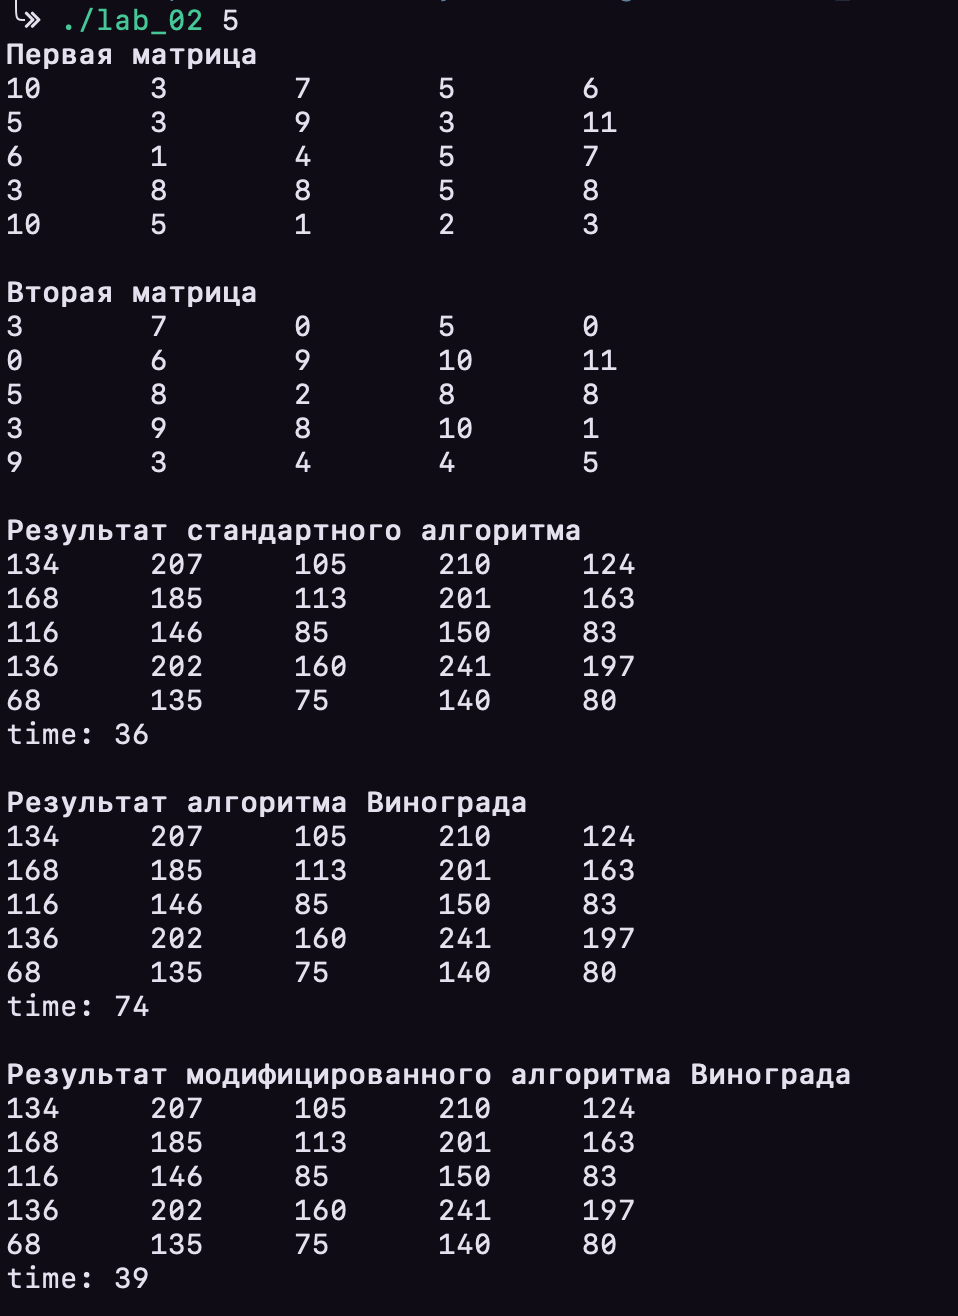
\includegraphics[scale=0.5]{one_arg}
    \caption{Один аргумент}
    \label{img:one-arg}
\end{figure}

\begin{figure}[H]
    \centering
    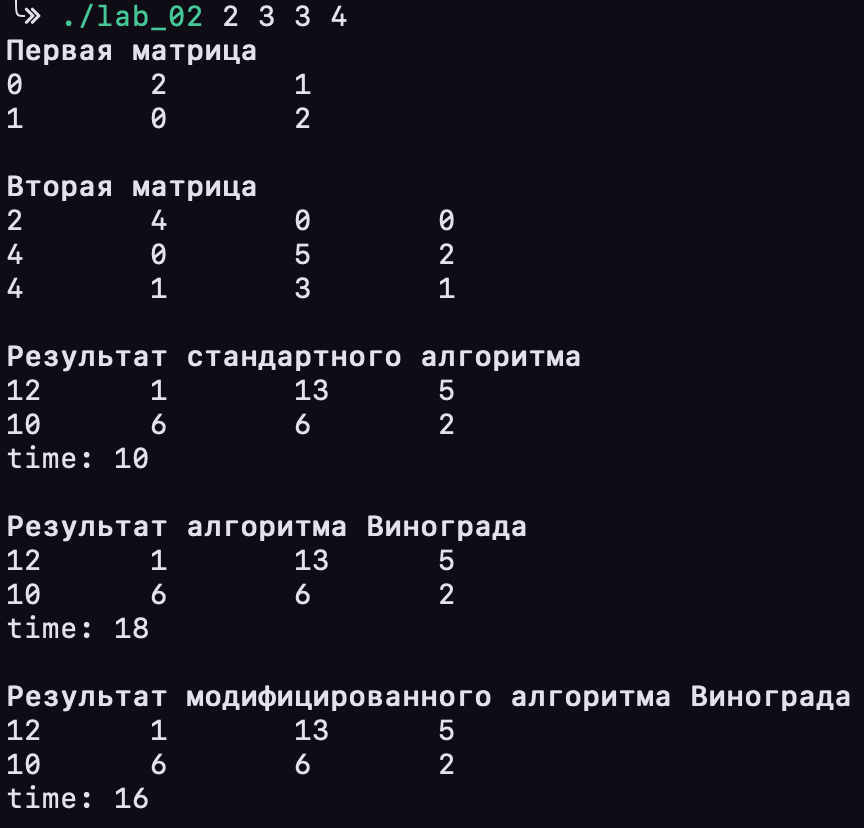
\includegraphics[scale=0.5]{four_arg}
    \caption{Четыре аргумента}
    \label{img:four-arg}
\end{figure}

\subsection{Результаты тестирования}

Для тестирования были использованы тесты из таблицы \ref{table:test}.
Результаты продемонстрированы на таблицах \ref{table:test-default},
\ref{table:test-vin}, \ref{table:test-modvin}.

\begin{table}[H]
    \caption{Результаты стандартного алгоритма}
    \label{table:test-default}
    \centering
    \begin{tabular}{|c|c|c|}
        \hline
        Первая матрца & Вторая матрица & Результат \\
        \hline
        1 2 & 1 2 & \ 7 10 \\
        3 4 & 3 4 & 15 22 \\
        \hline
        1 2 3 & 1 2 3 & \ 30\ \ 36\ \ 42 \\
        4 5 6 & 4 5 6 & \ 66\ \ 81\ \ 96 \\
        7 8 9 & 7 8 9 & 102 126 150 \\
        \hline
        1 2 3 & 1 & 14 \\
        4 5 6 & 2 & 32 \\
              & 3 & \\
        \hline
    \end{tabular}
\end{table}

\begin{table}[H]
    \caption{Результаты алгоримта Винограда}
    \label{table:test-vin}
    \centering
    \begin{tabular}{|c|c|c|}
        \hline
        Первая матрца & Вторая матрица & Результат \\
        \hline
        1 2 & 1 2 & \ 7 10 \\
        3 4 & 3 4 & 15 22 \\
        \hline
        1 2 3 & 1 2 3 & \ 30\ \ 36\ \ 42 \\
        4 5 6 & 4 5 6 & \ 66\ \ 81\ \ 96 \\
        7 8 9 & 7 8 9 & 102 126 150 \\
        \hline
        1 2 3 & 1 & 14 \\
        4 5 6 & 2 & 32 \\
              & 3 & \\
        \hline
    \end{tabular}
\end{table}

\begin{table}[H]
    \caption{Результаты оптимизированного алгоритма Винограда}
    \label{table:test-modvin}
    \centering
    \begin{tabular}{|c|c|c|}
        \hline
        Первая матрца & Вторая матрица & Результат \\
        \hline
        1 2 & 1 2 & \ 7 10 \\
        3 4 & 3 4 & 15 22 \\
        \hline
        1 2 3 & 1 2 3 & \ 30\ \ 36\ \ 42 \\
        4 5 6 & 4 5 6 & \ 66\ \ 81\ \ 96 \\
        7 8 9 & 7 8 9 & 102 126 150 \\
        \hline
        1 2 3 & 1 & 14 \\
        4 5 6 & 2 & 32 \\
              & 3 & \\
        \hline
    \end{tabular}
\end{table}

Все тесты пройдены успешно.

\subsection{Замеры времени}

На рисунке \ref{img:even} представлены результаты замера времени алгоритмов при
четных размерностях, а на рисунке \ref{img:noteven} при нечетных размерностях матриц.
Оба случая прогонялись на квардатных матрицах.

\begin{figure}[H]
    \begin{tikzpicture}
        \begin{axis}[
            legend pos = north west,
            xlabel=Размерность матрицы,
            ylabel=микросекунды,
            grid = major,
            width = 0.8\paperwidth,
            height = 0.38\paperheight,
            line width = 1
        ]
            \legend{
                Обычный алгоритм,
                Алгоритм Винограда,
                Оптимизированный алгоритм Винограда
            };
            \addplot[dashed] coordinates {
                (100, 34501)
                (200, 273438)
                (300, 911536)
                (400, 2287721)
                (500, 4467987)
                (600, 7982696)
                (700, 12589205)
                (800, 19543501)
                (900, 29907202)
                (1000, 39608083)
            };

            \addplot[black] coordinates {
                (100, 18468)
                (200, 141549)
                (300, 509012)
                (400, 1465966)
                (500, 2716895)
                (600, 4893372)
                (700, 7788205)
                (800, 11974361)
                (900, 17429652)
                (1000, 24443640)
            };

            \addplot[dotted] coordinates {
                (100, 15781)
                (200, 117581)
                (300, 438752)
                (400, 1146582)
                (500, 2466496)
                (600, 4238264)
                (700, 6635427)
                (800, 10541381)
                (900, 15063388)
                (1000, 21113694)
            };
        \end{axis}
    \end{tikzpicture}
    \caption{Четная размерность}
    \label{img:even}
\end{figure}

\begin{figure}[H]
    \begin{tikzpicture}
        \begin{axis}[
            legend pos = north west,
            xlabel=Размерность матрицы,
            ylabel=микросекунды,
            grid = major,
            width = 0.8\paperwidth,
            height = 0.38\paperheight,
            line width = 1
        ]
            \legend{
                Обычный алгоритм,
                Алгоритм Винограда,
                Оптимизированный алгоритм Винограда
            };
            \addplot[dashed] coordinates {
                (101, 34170)
                (201, 263159)
                (301, 909942)
                (401, 2262964)
                (501, 4486670)
                (601, 7851527)
                (701, 12517730)
                (801, 19429387)
                (901, 38556411)
                (1001, 62124826)
            };
            \addplot[black] coordinates {
                (101, 19163)
                (201, 142118)
                (301, 544590)
                (401, 1417500)
                (501, 2850727)
                (601, 4809657)
                (701, 7629622)
                (801, 12085389)
                (901, 17761017)
                (1001, 24574933)
            };
            \addplot[dotted] coordinates {
                (101, 15982)
                (201, 119376)
                (301, 442958)
                (401, 1257460)
                (501, 2437730)
                (601, 4266685)
                (701, 6876743)
                (801, 10731128)
                (901, 15011152)
                (1001, 23672051)
            };
        \end{axis}
    \end{tikzpicture}
    \caption{Нечетная размерность}
    \label{img:noteven}
\end{figure}

\subsection{Выводы}

Из графиков зависимости размерности матрицы ко времени ее вычисления
видно, что стандартный алгоритм работает медленне, чем алгоритм
Винограда на 50\%. Также, можно заметить, что оптимизация прошла
успешно и оптимизированный алгоритм Винограда работает быстрее
обычного на 5\%.

\newpage
\anonsection{Заключение}

В ходе данной работы было проведено сравнение стандартного алгоритма
умножения матриц с алгоритмом Винограда и его оптимизированной версией.
Данные алгоритмы широко применяются в математике, физике и
программировании.

Было проведено сравнение времени работы алгоритмов на случаях четной
размерности и нечетной размерности квадратной матрицы и сделаны
следующие выводы:

\begin{enumerate}
    \item стандартная реализация работаем медленнее алгоритма Винограда
        на 50\%;
    \item оптимизированная версия алгоримта Винограда работает быстрее
        обычной на 5\%.
\end{enumerate}

Все цели, поставленные на эту работы, были выполнены:

\begin{enumerate}
    \item реализованы алгоритмы умножения матриц;
    \item проведен сравнительный анализ стандартного алгоритма и улучшенных алгоритмов по
        затрачиваемым ресурсам;
    \item проведено экспериментальное подтверждение различий во временной эффективности
        сравниваемых алгоритмов.
\end{enumerate}

\newpage
\addcontentsline{toc}{section}{Список используемой литературы}

\begin{thebibliography}{}
    \bibitem{haskell} Анисимов Н.С. и Строганов Ю.В. - "Реализация алгоритма умножения матриц по Винограду"
на языке Haskell
    \bibitem{litr} Корн Г., Корн Т. - "Алгебра матриц и матричное исчисление"
    \bibitem{chrono} Документация по chrono [Электронный ресурс]. -  Режим доступа: http://www.cplusplus.com/reference/chrono/ Дата обращения: 08.10.2019
\end{thebibliography}

\end{document}
